\documentclass{beamer}
\usetheme[pageofpages=of,% String used between the current page and the
                         % total page count.
          bullet=circle,% Use circles instead of squares for bullets.
          titleline=true,% Show a line below the frame title.
          alternativetitlepage=true,% Use the fancy title page.
       %   titlepagelogo=logo-polito,% Logo for the first page.
       %   watermark=watermark-polito,% Watermark used in every page.
       %   watermarkheight=100px,% Height of the watermark.
       %   watermarkheightmult=4,% The watermark image is 4 times bigger
                                % than watermarkheight.
          ]{Torino}

\setbeamertemplate{footline}{
  \begin{beamercolorbox}[wd=\paperwidth,ht=1ex,dp=1ex]{footline}
    \vspace{5pt} \hspace{1em} \insertframenumber/\inserttotalframenumber
  \end{beamercolorbox}
}

\author{Brendon J. Brewer}
\title{STATS 331 -- Introduction to Bayesian Statistics}
\institute{The University of Auckland}
\date{}


\linespread{1.3}
\usepackage{minted}
\usepackage[utf8]{inputenc}
\usepackage{dsfont}
\newcommand{\given}{\,|\,}


\begin{document}

\frame{\titlepage}

\begin{frame}
\centering
\Large
Other Regression Models

\end{frame}


\begin{frame}
\frametitle{Other Regression Models}
We will now look at how to implement some other regression models
(`GLMs', taught classically in STATS 330) in JAGS.
We will do the following, which are really just different choices for
what to use for the sampling distribution:

\begin{itemize}
\item Logistic regression \pause
\item Poisson regression \pause
\item Negative binomial regression
\end{itemize}

\end{frame}


\begin{frame}
\frametitle{Logistic Regression Example}
\begin{itemize}
\item For logistic regression, we will look at a simple example with one
explanatory variable. The extension to more explanatory variables should be
clear.\pause
\item In this data, the explanatory variable is the age (of a patient)
and the response variable is 0 (no heart disease) or 1 (heart disease).
\end{itemize}

\end{frame}

\begin{frame}
\frametitle{Logistic Regression Example}

\begin{center}
\includegraphics[width=0.7\textwidth]{images/chd_data.pdf}
\end{center}

\end{frame}

\begin{frame}
\frametitle{Logistic Regression Assumptions}
We assume that the probability of having heart disease is some function of the
explanatory variables. Based on those probabilities,
the data have a Bernoulli distribution.
\end{frame}

\begin{frame}
\frametitle{Logits}
Logits are a transformed version of probabilities that live in
$(-\infty, \infty)$ instead of $[0, 1]$. The definition of a logit $\ell$
in terms of a probability $p$ is
\begin{align}
\ell &= \log\left(\frac{p}{1-p}\right).
\end{align}
\pause
The inverse, to convert a logit $\ell$ to a probability $p$
is the `logistic function':
\begin{align}
p &= \frac{e^\ell}{1 + e^\ell} = \frac{1}{1 + e^{-\ell}}.
\end{align}

\end{frame}

\begin{frame}
\frametitle{Logistic Regression Assumptions}

\begin{align}
\ell_i &= \beta_0 + \beta_1 x_i \\
p_i &= \frac{1}{1 + e^{-\ell_i}}\\
y_i \given \beta_0, \beta_1 &\sim \textnormal{Bernoulli}\left(p_i\right).
\end{align}
\pause

Usefully, to write this in JAGS, we don't need to write down the logistic
equation manually.

\end{frame}


\begin{frame}[fragile]
\frametitle{Logistic Regression: JAGS Code}

\begin{minted}{r}
model
{
    beta0 ~ dunif(-1000, 1000)
    beta1 ~ dunif(-1000, 1000)

    for(i in 1:length(y))
    {
        logit(p[i]) <- beta0 + beta1*(x[i] - mean(x))
        y[i] ~ dbern(p[i])
    }
}
\end{minted}

\end{frame}

\begin{frame}[fragile]
\frametitle{Logistic Regression: Prediction}
We can do prediction just as we did in the linear regression case,
by adding nodes for \mintinline{r}{y_new}. The posterior mean of it
will give the posterior probability that $y_{\rm new} = 1$.\\[0.5em]\pause

We could also just take the posterior mean of $p_{\rm new}$.
\end{frame}


\begin{frame}[fragile]
\frametitle{Logistic Regression: Plotting}

\begin{minted}{r}
plot(data$x, data$y, xlab="Age", ylab="Disease")
x = seq(10, 100, by=0.1)
rows = sample(1:nrow(results), 100)
for(row in rows)
{
    l = results$beta0[row] +
        results$beta1[row]*(x - mean(data$x))
    p = 1/(1 + exp(-l))
    lines(x, p, col=rgb(0, 0, 0, 0.1))
}
\end{minted}

\end{frame}

\begin{frame}
\frametitle{Logistic Regression: Plotting}

\begin{center}
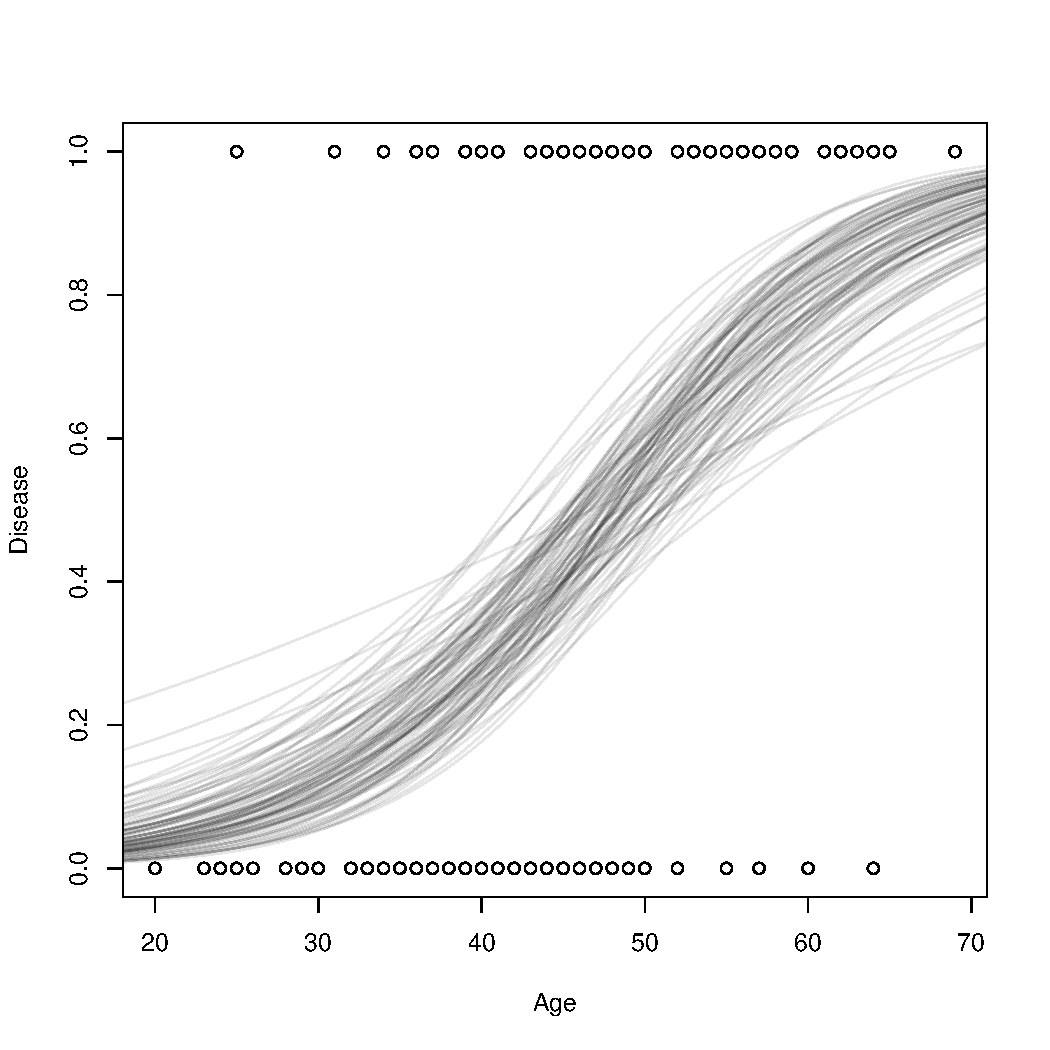
\includegraphics[width=0.6\textwidth]{images/logistic_curves.pdf}
\end{center}

\end{frame}


\end{document}

